%%%%%%%%%%%%%%%%%%%%%%%%%%%%%%%%%%%%%%%%%%%%%%%%%%%%%%%%%%%%%%%%%%%%%%%%%%%%%%%%%%%%%%%%%%%%%%%%%%%%%%%%%%%%%%%%%%%%%%%%%%%%%%%%%%%%%%%%%%%%%%%%%%%%%%%%%%%%%%%%%%%
% Written By Michael Brodskiy
% Class: Embedded Design: Enabling Robotics
% Professor: S. Shazli
%%%%%%%%%%%%%%%%%%%%%%%%%%%%%%%%%%%%%%%%%%%%%%%%%%%%%%%%%%%%%%%%%%%%%%%%%%%%%%%%%%%%%%%%%%%%%%%%%%%%%%%%%%%%%%%%%%%%%%%%%%%%%%%%%%%%%%%%%%%%%%%%%%%%%%%%%%%%%%%%%%%

\include{Includes.tex}

\pagestyle{fancy}

\title{Embedded Systems}
\date{\today}
\author{Michael Brodskiy\\ \small Professor: S. Shazli}

\begin{document}

\maketitle

\thispagestyle{fancy}

\begin{itemize}

  \item A computer system embedded into another system

    \begin{itemize} 

      \item Constraints from external input/output 

      \item Application-specific

        \begin{itemize} 

          \item Diverse set of application areas

        \end{itemize}

    \end{itemize}

  \item Abstraction

    \begin{itemize}

      \item Productivity enhancer — don't need to worry about details\ldots

        \begin{itemize}

          \item A car can be driven without the knowledge of how an internal combustion engine works

        \end{itemize}

      \item \ldots until something goes wrong

        \begin{itemize}

          \item Where's the dipstick? What's a spark plug? Am I out of gas?

        \end{itemize}

      \item Important to understand the components and how they work together

    \end{itemize}

  \item Hardware vs. Software

    \begin{itemize}

      \item All computers, given enough time and memory, are capable of computing the same exact things

      \item In theory, computers ``compute'' anything that's possible to compute

        \begin{itemize}

          \item Given enough memory and time

        \end{itemize}

      \item In practice, ``solving problems'' involves computing under constraints

        \begin{itemize}

          \item Time

            \begin{itemize}

              \item Weather forecast, next frame animation, \ldots

            \end{itemize}

          \item Cost

            \begin{itemize}

              \item iPod, automotive engine controller, \ldots

            \end{itemize}

          \item Power

            \begin{itemize}

              \item Smartphone, tablet, \ldots

            \end{itemize}

        \end{itemize}

    \end{itemize}

  \item Layers of Abstraction

    \begin{center}
      \begin{tabular}[h]{|c|}
        \hline
        Problems\\
        \hline
        Algorithms\\
        \hline
        Language\\
        \hline
        Instruction Set Architecture\\
        \hline
        Microarchitecture\\
        \hline
        Circuits\\
        \hline
        Devices\\
        \hline
      \end{tabular}
    \end{center}

    \begin{itemize}

      \item Problem Statement

        \begin{itemize}

          \item Stated using ``natural language''

          \item May be ambiguous, imprecise

        \end{itemize}

      \item Algorithm

        \begin{itemize}

          \item Step-by-step procedure, recipe, guaranteed to finish

          \item Definiteness, effective computability, finiteness

        \end{itemize}

      \item Program

        \begin{itemize}

          \item Express the algorithm using a computer language

          \item High-level language, low-level language

        \end{itemize}

      \item Instruction Set Architecture (ISA)

        \begin{itemize}

          \item Specifies the set of instructions the computer can perform

          \item Data types, addressing mode, hardware/software interface

        \end{itemize}

      \item Microarchitecture

        \begin{itemize}

          \item Detailed organization of a processor implementation

          \item Different implementations of a single ISA

        \end{itemize}

      \item Logic Circuits

        \begin{itemize}

          \item Combine basic operations to realize microarchitecture

        \end{itemize}

      \item Problem to algorithm is solved by software design, algorithm to program through programming, and program to instruction set architecture through compilation/interpretation

      \item Instruction set architecture to microarchitecture is solved through processor design, microarchitecture to a circuit is solved through logic/circuit design, and a circuit to a device is solved through the engineering process and fabrication

    \end{itemize}

    \begin{figure}[h!]
      \centering
      \tikzset{every picture/.style={line width=0.75pt}} %set default line width to 0.75pt        

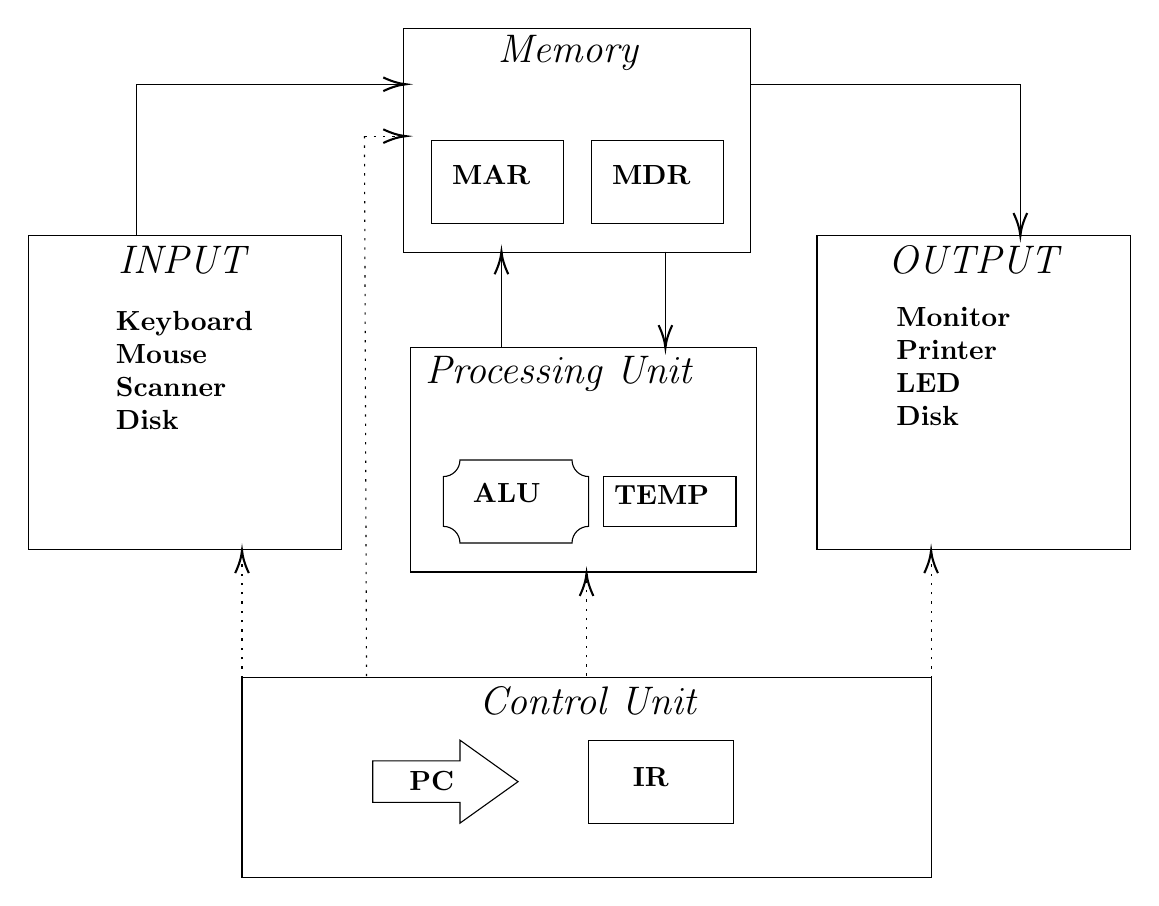
\begin{tikzpicture}[x=0.75pt,y=0.75pt,yscale=-1,xscale=1]
%uncomment if require: \path (0,536); %set diagram left start at 0, and has height of 536

%Shape: Square [id:dp6842021214778704] 
\draw   (38,107) -- (189,107) -- (189,258) -- (38,258) -- cycle ;
%Shape: Square [id:dp2846781522874837] 
\draw   (418,107) -- (569,107) -- (569,258) -- (418,258) -- cycle ;
%Shape: Rectangle [id:dp7000294601399879] 
\draw   (141,320) -- (473,320) -- (473,416) -- (141,416) -- cycle ;
%Right Arrow [id:dp27948617576185875] 
\draw   (204,360) -- (246,360) -- (246,350) -- (274,370) -- (246,390) -- (246,380) -- (204,380) -- cycle ;
%Shape: Rectangle [id:dp5238183889968957] 
\draw   (308,350) -- (378,350) -- (378,390) -- (308,390) -- cycle ;
%Shape: Rectangle [id:dp4274195934195226] 
\draw   (222,161) -- (389,161) -- (389,269) -- (222,269) -- cycle ;
%Shape: Rectangle [id:dp8158827848725543] 
\draw   (219,7) -- (386,7) -- (386,115) -- (219,115) -- cycle ;
%Shape: Rectangle [id:dp5804130759863328] 
\draw   (232.5,61) -- (296,61) -- (296,101) -- (232.5,101) -- cycle ;
%Shape: Rectangle [id:dp12227146904878561] 
\draw   (309.5,61) -- (373,61) -- (373,101) -- (309.5,101) -- cycle ;
%Shape: Plaque [id:dp995424536451063] 
\draw   (238,223) .. controls (242.42,223) and (246,219.42) .. (246,215) -- (300,215) .. controls (300,219.42) and (303.58,223) .. (308,223) -- (308,247) .. controls (303.58,247) and (300,250.58) .. (300,255) -- (246,255) .. controls (246,250.58) and (242.42,247) .. (238,247) -- cycle ;
%Shape: Rectangle [id:dp6361147141573973] 
\draw   (315,223) -- (379,223) -- (379,247) -- (315,247) -- cycle ;
%Straight Lines [id:da8084212324067266] 
\draw  [dash pattern={on 0.84pt off 2.51pt}]  (141,320) -- (141,260.58) ;
\draw [shift={(141,258.58)}, rotate = 90] [color={rgb, 255:red, 0; green, 0; blue, 0 }  ][line width=0.75]    (10.93,-3.29) .. controls (6.95,-1.4) and (3.31,-0.3) .. (0,0) .. controls (3.31,0.3) and (6.95,1.4) .. (10.93,3.29)   ;
%Straight Lines [id:da4139933874047299] 
\draw  [dash pattern={on 0.84pt off 2.51pt}]  (473,320) -- (473,260.58) ;
\draw [shift={(473,258.58)}, rotate = 90] [color={rgb, 255:red, 0; green, 0; blue, 0 }  ][line width=0.75]    (10.93,-3.29) .. controls (6.95,-1.4) and (3.31,-0.3) .. (0,0) .. controls (3.31,0.3) and (6.95,1.4) .. (10.93,3.29)   ;
%Straight Lines [id:da6375241441773398] 
\draw  [dash pattern={on 0.84pt off 2.51pt}]  (307,319) -- (307,271.58) ;
\draw [shift={(307,269.58)}, rotate = 90] [color={rgb, 255:red, 0; green, 0; blue, 0 }  ][line width=0.75]    (10.93,-3.29) .. controls (6.95,-1.4) and (3.31,-0.3) .. (0,0) .. controls (3.31,0.3) and (6.95,1.4) .. (10.93,3.29)   ;
%Straight Lines [id:da7823928920015608] 
\draw  [dash pattern={on 0.84pt off 2.51pt}]  (200,59) -- (201,320) ;
%Straight Lines [id:da0832406275103772] 
\draw  [dash pattern={on 0.84pt off 2.51pt}]  (200,59) -- (218,59) ;
\draw [shift={(220,59)}, rotate = 180] [color={rgb, 255:red, 0; green, 0; blue, 0 }  ][line width=0.75]    (10.93,-3.29) .. controls (6.95,-1.4) and (3.31,-0.3) .. (0,0) .. controls (3.31,0.3) and (6.95,1.4) .. (10.93,3.29)   ;
%Straight Lines [id:da6550156642776477] 
\draw    (266,161) -- (266,116.58) ;
\draw [shift={(266,114.58)}, rotate = 90] [color={rgb, 255:red, 0; green, 0; blue, 0 }  ][line width=0.75]    (10.93,-3.29) .. controls (6.95,-1.4) and (3.31,-0.3) .. (0,0) .. controls (3.31,0.3) and (6.95,1.4) .. (10.93,3.29)   ;
%Shape: Boxed Line [id:dp25364397431402463] 
\draw    (345,114.58) -- (345,159) ;
\draw [shift={(345,161)}, rotate = 270] [color={rgb, 255:red, 0; green, 0; blue, 0 }  ][line width=0.75]    (10.93,-3.29) .. controls (6.95,-1.4) and (3.31,-0.3) .. (0,0) .. controls (3.31,0.3) and (6.95,1.4) .. (10.93,3.29)   ;
%Straight Lines [id:da5907462027159831] 
\draw    (90,34) -- (90,107) ;
%Straight Lines [id:da14006758297346078] 
\draw    (90,34) -- (218,34) ;
\draw [shift={(220,34)}, rotate = 180] [color={rgb, 255:red, 0; green, 0; blue, 0 }  ][line width=0.75]    (10.93,-3.29) .. controls (6.95,-1.4) and (3.31,-0.3) .. (0,0) .. controls (3.31,0.3) and (6.95,1.4) .. (10.93,3.29)   ;
%Straight Lines [id:da5528848956046384] 
\draw    (516,34) -- (516,105) ;
\draw [shift={(516,107)}, rotate = 270] [color={rgb, 255:red, 0; green, 0; blue, 0 }  ][line width=0.75]    (10.93,-3.29) .. controls (6.95,-1.4) and (3.31,-0.3) .. (0,0) .. controls (3.31,0.3) and (6.95,1.4) .. (10.93,3.29)   ;
%Straight Lines [id:da4578186118418053] 
\draw    (516,34) -- (386,34) ;

% Text Node
\draw (80,111) node [anchor=north west][inner sep=0.75pt]   [align=left] {\textit{{\Large INPUT}}};
% Text Node
\draw (79,142) node [anchor=north west][inner sep=0.75pt]   [align=left] {\textbf{Keyboard}\\\textbf{Mouse}\\\textbf{Scanner}\\\textbf{Disk}};
% Text Node
\draw (451,111) node [anchor=north west][inner sep=0.75pt]   [align=left] {\textit{{\Large OUTPUT}}};
% Text Node
\draw (455,140) node [anchor=north west][inner sep=0.75pt]   [align=left] {\textbf{Monitor}\\\textbf{Printer}\\\textbf{LED}\\\textbf{Disk}};
% Text Node
\draw (254,323) node [anchor=north west][inner sep=0.75pt]   [align=left] {\textit{{\Large Control Unit}}};
% Text Node
\draw (232.42,369.5) node   [align=left] {\textbf{PC}};
% Text Node
\draw (328,362) node [anchor=north west][inner sep=0.75pt]   [align=left] {\textbf{IR}};
% Text Node
\draw (228,164) node [anchor=north west][inner sep=0.75pt]   [align=left] {{\Large \textit{Processing Unit}}};
% Text Node
\draw (263,9) node [anchor=north west][inner sep=0.75pt]   [align=left] {{\Large \textit{Memory}}};
% Text Node
\draw (241,72) node [anchor=north west][inner sep=0.75pt]   [align=left] {\textbf{MAR}};
% Text Node
\draw (318,72) node [anchor=north west][inner sep=0.75pt]   [align=left] {\textbf{MDR}};
% Text Node
\draw (251,225) node [anchor=north west][inner sep=0.75pt]   [align=left] {\textbf{ALU}};
% Text Node
\draw (319,226) node [anchor=north west][inner sep=0.75pt]   [align=left] {\textbf{TEMP}};


\end{tikzpicture}

      \caption{Processing System Flowchart}
      \label{fig:1}
    \end{figure}

  \item Basic Building Blocks

    \begin{itemize}

      \item Electrons

      \item Transistors

      \item Logic Gates

      \item Combinational Logic Circuits

      \item Sequential Logic Circuits

        \begin{itemize}

          \item Storage Elements and Memory

        \end{itemize}

      \item Cores

      \item Memories

      \item Caches

    \end{itemize}

\end{itemize}

\end{document}

